% ===========================================================================
% Part IX - Margin-Based Learning: Support Vector Machines (Experiment 17)
% ===========================================================================

\part{Margin-Based Learning: Support Vector Machines}

% ---------------------------------------------------------------------------
\chapter{Experiment 17: Support Vector Machine (SVM)}\label{exp:17}

\quickfacts
  {Dataset}{Breast Cancer (569 $\times$ 30; 2 features for the kernel view, all 30 for accuracy) and Old Faithful geyser (\texttt{data/geyser.csv}, 272 eruptions)}
  {Key parameters}{SVC: RBF kernel, C = 1.0, gamma = `scale'; SVR: RBF, C = 10, $\varepsilon$ = 0.3}
  {Headline result}{SVC accuracy 0.9790 (96/426 support vectors); SVR $R^2$ 0.8968 (103/272 support vectors)}

\section{Objective}
Train SVM classifiers and investigate the effects of kernel, $C$ and $\gamma$; demonstrate
Support Vector Regression with an $\varepsilon$-insensitive tube.

\section{Suggested Dataset}
(a) Breast Cancer (569 $\times$ 30): two features (mean radius, mean texture) for the 2D
kernel view and all 30 features for the accuracy benchmark. (b) Old Faithful geyser
(\texttt{data/geyser.csv}, 272 eruptions) for SVR.

\section{Required Libraries}
scikit-learn, numpy, pandas, matplotlib.

\section{Brief Theory}
\textbf{SVC (soft margin)} solves
\[
\min_{w,b,\xi}\ \tfrac{1}{2}\lVert w\rVert^2 + C\sum_i \xi_i
\quad\text{s.t.}\quad y_i\bigl(w^T\phi(x_i)+b\bigr) \ge 1-\xi_i,\ \ \xi_i \ge 0 .
\]
The dual problem depends only on inner products $K(x_i, x_j)$, which enables the
\textbf{kernel trick}: compute similarities in a high-dimensional feature space without mapping
the data there explicitly. The solution is sparse --- only points with $\alpha_i > 0$
(\textbf{support vectors}) define the boundary. Kernels used here: linear $x^Tz$, polynomial
$(\gamma x^Tz + r)^d$ and RBF $\exp(-\gamma\lVert x-z\rVert^2)$. $C$ penalizes margin
violations; $\gamma$ controls the RBF width. \textbf{SVR} applies the same machinery to
regression with an \textbf{$\varepsilon$-insensitive tube}: residuals within $\pm\varepsilon$
cost nothing and only points outside the tube become support vectors.

\section{Procedure}
\begin{enumerate}
  \item Scale the features.
  \item Train SVC with linear, polynomial and RBF kernels on two breast-cancer features; plot
        the boundaries, margins and support vectors.
  \item Train the RBF SVC on all 30 features; report accuracy and the support-vector count.
  \item Fit SVR (RBF, $C = 10$, $\varepsilon = 0.3$) to the Old Faithful data (waiting time
        $\rightarrow$ eruption duration); plot the fitted curve and the tube.
  \item Report $R^2$, RMSE and the support-vector share.
\end{enumerate}

\section{Reference Implementation}
\begin{lstlisting}[style=mlcode,caption={SVC per kernel and SVR with an epsilon-insensitive tube}]
clf = SVC(kernel=k_name, C=1.0, gamma='scale', degree=3, random_state=42).fit(X_2d_scaled, y_2d)
svc_rbf = SVC(kernel='rbf', C=1.0, random_state=42).fit(X_train_c_s, y_train_c)
svr_model = SVR(kernel='rbf', C=10.0, epsilon=0.3, gamma='scale').fit(X_svr_scaled, y_svr)
\end{lstlisting}

\section{Evaluation / Expected Output}
\begin{table}[htbp]
  \centering
  \caption{SVM results on the two real datasets.}
  \begin{tabular}{@{}llr@{}}
    \toprule
    \textbf{Experiment} & \textbf{Metric} & \textbf{Value} \\
    \midrule
    SVC (RBF, 30 features) & Test accuracy & \best{0.9790} \\
    SVC (RBF, 30 features) & Support vectors & 96 of 426 (22.5\%) \\
    SVR (Old Faithful) & $R^2$ & 0.8968 \\
    SVR (Old Faithful) & RMSE & 0.366 minutes \\
    SVR (Old Faithful) & Support vectors & 103 of 272 (37.9\%) \\
    \bottomrule
  \end{tabular}
\end{table}

\begin{figure}[htbp]
  \centering
  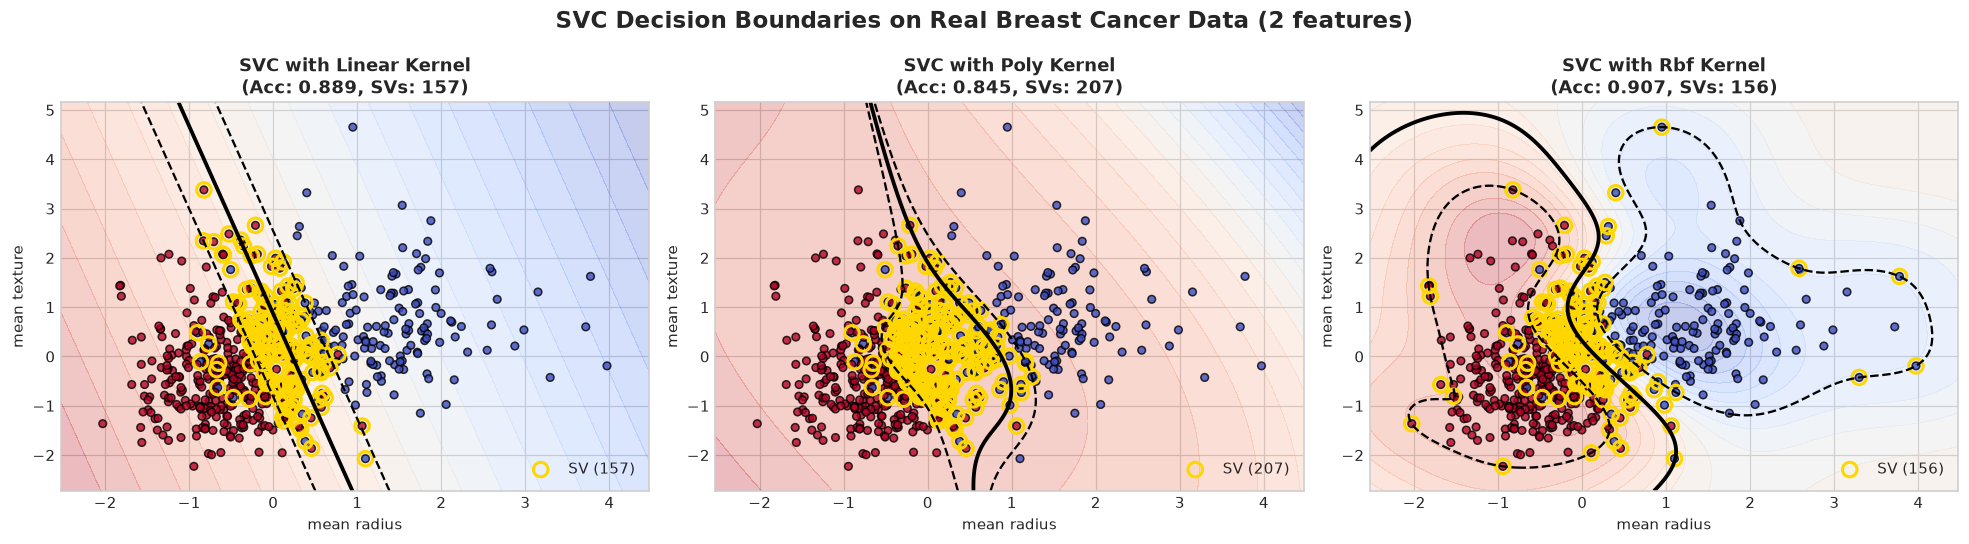
\includegraphics[width=0.98\textwidth]{figures/exp17_svc_kernels.png}
  \caption{SVC decision boundaries, margins and support vectors on two real breast-cancer
  features for the linear, polynomial and RBF kernels.}
  \label{fig:exp17-kernels}
\end{figure}

\begin{figure}[htbp]
  \centering
  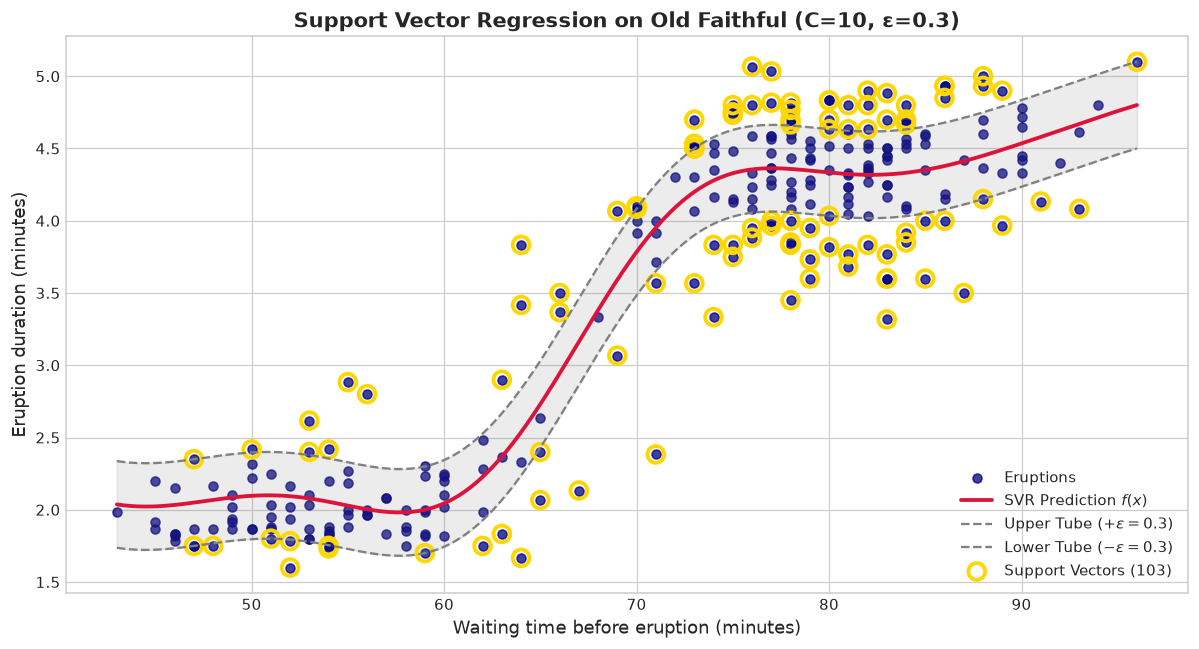
\includegraphics[width=0.85\textwidth]{figures/exp17_svr_tube.png}
  \caption{Support Vector Regression on the Old Faithful geyser with the $\varepsilon = 0.3$
  tube; highlighted points are support vectors.}
  \label{fig:exp17-svr}
\end{figure}

The 2D kernel figure shows the linear kernel underfitting the real diagnostic data while the
polynomial and RBF kernels produce curved boundaries. The RBF SVC reaches 0.9790 accuracy with
only 96 of 426 training points as support vectors --- about 77\% of the data could be discarded
without changing the classifier. The geyser scatter is bimodal (short and long eruptions); the
RBF SVR smoothly bridges the two modes and the tube leaves most residuals unpenalized.

\section{Viva / Discussion Questions}
\begin{description}
  \item[What is a support vector?] A training point on or inside the margin ($\alpha > 0$) that
  alone defines the decision boundary.
  \item[Effect of $C$?] Large $C$ penalizes violations strongly (narrow margin, possible
  overfitting); small $C$ allows a wider margin and more violations.
  \item[Effect of $\gamma$?] Large $\gamma$ makes each point's influence local (wiggly
  boundary); small $\gamma$ makes the RBF smoother, approaching a linear model.
  \item[What is the kernel trick?] Computing inner products in a high-dimensional feature
  space without explicitly mapping the points there.
  \item[What is the $\varepsilon$-tube in SVR?] The zero-loss zone around the fitted function;
  only points outside it become support vectors. A wider tube (0.3 vs.\ 0.1) reduced the
  support-vector count with the same $R^2$.
  \item[Why does SVM require careful scaling?] Margins and kernels use Euclidean distances;
  unscaled features with larger ranges dominate them and degrade the fit.
\end{description}

\section{Complete Code Listing}
% ===========================================================================
% exp17_svm.tex - complete code listings for Experiment 17
% Source: notebooks/09_support_vector_machine.ipynb (executed)
% ===========================================================================

\begin{lstlisting}[style=mlcode,caption={Core numerical and plotting libraries}]
# ---- Core numerical and plotting libraries ----
import numpy as np
import pandas as pd
import matplotlib.pyplot as plt
import seaborn as sns

# ---- Dataset + model selection ----
from sklearn.datasets import load_breast_cancer
from sklearn.model_selection import train_test_split
from sklearn.preprocessing import StandardScaler
# ---- SVM models: classification and regression ----
from sklearn.svm import SVC, SVR
# ---- Evaluation metrics ----
from sklearn.metrics import r2_score, root_mean_squared_error

# Styling setup (consistent look across all notebooks)
plt.style.use('seaborn-v0_8-whitegrid' if 'seaborn-v0_8-whitegrid' in plt.style.available else 'default')
plt.rcParams['font.sans-serif'] = 'DejaVu Sans'
plt.rcParams['figure.figsize'] = (10, 6)
plt.rcParams['figure.dpi'] = 110

np.random.seed(42)
print("SVM modules loaded successfully!")
\end{lstlisting}

\begin{lstlisting}[style=mlcode,caption={2D real data for visualizing margins and kernels}]
# ---- 2D real data for visualizing margins and kernels ----
# Two diagnostic measurements from the Breast Cancer dataset (malignant vs benign).
cancer_2d = load_breast_cancer()
X_2d = cancer_2d.data[:, [0, 1]]    # mean radius and mean texture
y_2d = cancer_2d.target
feature_names_2d = ['mean radius', 'mean texture']

scaler_2d = StandardScaler()
X_2d_scaled = scaler_2d.fit_transform(X_2d)

kernels = ['linear', 'poly', 'rbf']
fig, axes = plt.subplots(1, 3, figsize=(18, 5))

# Coordinate grid used to draw the decision boundary as a contour
x_min, x_max = X_2d_scaled[:, 0].min() - 0.5, X_2d_scaled[:, 0].max() + 0.5
y_min, y_max = X_2d_scaled[:, 1].min() - 0.5, X_2d_scaled[:, 1].max() + 0.5
xx, yy = np.meshgrid(np.linspace(x_min, x_max, 200), np.linspace(y_min, y_max, 200))

for ax, k_name in zip(axes, kernels):
    # Train one SVC per kernel on the same real data
    clf = SVC(kernel=k_name, C=1.0, gamma='scale', degree=3, random_state=42)
    clf.fit(X_2d_scaled, y_2d)

    # Signed distance to the hyperplane for every grid point
    Z = clf.decision_function(np.c_[xx.ravel(), yy.ravel()]).reshape(xx.shape)

    # Filled contour = decision regions; solid line = boundary (Z=0); dashed = margins (Z=±1)
    ax.contourf(xx, yy, Z, levels=np.linspace(Z.min(), Z.max(), 20), cmap='coolwarm', alpha=0.3)
    ax.contour(xx, yy, Z, levels=[-1.0, 0.0, 1.0], linestyles=['--', '-', '--'], colors=['k', 'k', 'k'], linewidths=[1.5, 2.5, 1.5])

    # Scatter the data points (colored by class)
    ax.scatter(X_2d_scaled[:, 0], X_2d_scaled[:, 1], c=y_2d, cmap='coolwarm', edgecolors='k', s=25, alpha=0.8)

    # Highlight the support vectors (the points that define the margin)
    sv = clf.support_vectors_
    ax.scatter(sv[:, 0], sv[:, 1], s=90, facecolors='none', edgecolors='gold', linewidths=2.0, label=f'SV ({len(sv)})')

    ax.set_title(f"SVC with {k_name.capitalize()} Kernel\n(Acc: {clf.score(X_2d_scaled, y_2d):.3f}, SVs: {len(sv)})", fontweight='bold')
    ax.set_xlabel(feature_names_2d[0])
    ax.set_ylabel(feature_names_2d[1])
    ax.legend(loc='lower right')

plt.suptitle("SVC Decision Boundaries on Real Breast Cancer Data (2 features)", fontsize=15, fontweight='bold')
plt.tight_layout()
plt.show()
\end{lstlisting}

\begin{lstlisting}[style=mlcode,caption={SVC on a real dataset: Breast Cancer (RBF kernel)}]
# ---- SVC on a real dataset: Breast Cancer (RBF kernel) ----
cancer = load_breast_cancer()
X_train_c, X_test_c, y_train_c, y_test_c = train_test_split(
    cancer.data, cancer.target, test_size=0.25, random_state=42, stratify=cancer.target
)
scaler_c = StandardScaler()
X_train_c_s = scaler_c.fit_transform(X_train_c)
X_test_c_s = scaler_c.transform(X_test_c)

svc_rbf = SVC(kernel='rbf', C=1.0, random_state=42)
svc_rbf.fit(X_train_c_s, y_train_c)
print(f"SVC (RBF) test accuracy on Breast Cancer: {svc_rbf.score(X_test_c_s, y_test_c):.4f}")
print(f"Support vectors used: {len(svc_rbf.support_)} of {len(X_train_c)} training samples")
\end{lstlisting}

\begin{lstlisting}[style=mlcode,caption={Real 1D regression: Old Faithful geyser}]
# ---- Real 1D regression: Old Faithful geyser ----
# x = waiting time before an eruption (minutes), y = eruption duration (minutes)
geyser = pd.read_csv('../data/geyser.csv')
X_svr = geyser['waiting'].values.reshape(-1, 1)
y_svr = geyser['eruptions'].values
print(f"Old Faithful: {len(geyser)} eruptions | waiting {X_svr.min()}-{X_svr.max()} min | duration {y_svr.min()}-{y_svr.max()} min")

# Scale the feature (SVR is distance-based); the target stays in minutes for interpretability
scaler_svr = StandardScaler()
X_svr_scaled = scaler_svr.fit_transform(X_svr)

# epsilon defines the width of the "no penalty" tube around the prediction (in minutes)
epsilon_val = 0.3
svr_model = SVR(kernel='rbf', C=10.0, epsilon=epsilon_val, gamma='scale')
svr_model.fit(X_svr_scaled, y_svr)

# Dense grid for drawing a smooth prediction curve, converted back to minutes
X_grid = np.linspace(X_svr_scaled.min(), X_svr_scaled.max(), 300).reshape(-1, 1)
y_grid_pred = svr_model.predict(X_grid)
X_grid_orig = scaler_svr.inverse_transform(X_grid).ravel()

# Support vectors = training points that lie on/outside the epsilon tube
sv_indices = svr_model.support_
X_sv = X_svr[sv_indices]
y_sv = y_svr[sv_indices]

plt.figure(figsize=(11, 6))
# Training samples
plt.scatter(X_svr, y_svr, color='navy', s=35, alpha=0.75, label='Eruptions')

# Regression surface
plt.plot(X_grid_orig, y_grid_pred, color='crimson', lw=2.5, label='SVR Prediction $f(x)$')

# Epsilon-insensitive tube boundaries + shaded tube
plt.plot(X_grid_orig, y_grid_pred + epsilon_val, color='gray', linestyle='--', lw=1.5, label=rf'Upper Tube ($+\epsilon={epsilon_val}$)')
plt.plot(X_grid_orig, y_grid_pred - epsilon_val, color='gray', linestyle='--', lw=1.5, label=rf'Lower Tube ($-\epsilon={epsilon_val}$)')
plt.fill_between(X_grid_orig, y_grid_pred - epsilon_val, y_grid_pred + epsilon_val, color='gray', alpha=0.15)

# Support vectors are highlighted - only these points influence the fitted curve
plt.scatter(X_sv, y_sv, s=120, facecolors='none', edgecolors='gold', linewidths=2.5, label=f'Support Vectors ({len(X_sv)})')

plt.title(f"Support Vector Regression on Old Faithful (C=10, ε={epsilon_val})", fontsize=14, fontweight='bold')
plt.xlabel("Waiting time before eruption (minutes)", fontsize=12)
plt.ylabel("Eruption duration (minutes)", fontsize=12)
plt.legend(loc='lower right')
plt.tight_layout()
plt.show()

# ---- Quantitative evaluation ----
print(f"SVR R² Score: {r2_score(y_svr, svr_model.predict(X_svr_scaled)):.4f}")
print(f"SVR RMSE:     {root_mean_squared_error(y_svr, svr_model.predict(X_svr_scaled)):.4f} minutes")
print(f"Support Vectors: {len(X_sv)} out of {len(X_svr)} points ({len(X_sv)/len(X_svr)*100:.1f}%)")
\end{lstlisting}

